\section{SD卡的驱动框架}

\subsection{SD/MMC卡介绍}

\subsubsection{什么是MMC卡}

MMC是MultiMediaCard的缩写,即多媒体卡。它是一种非易失性存储器件,体积小巧(24mm*32mm*1.4mm),容量大,耗电量低,传输速度快,广泛应用于消费类电子产品中。

\subsubsection{什么是SD卡}

SD卡为Secure Digital Memory Card, 即安全数码卡。它在MMC的基础上发展而来,增加了两个主要特色:SD卡强调数据的安全安全,可以设定所储存的使用权限,防止数据被他人复制;另外一个特色就是传输速度比2.11版的MMC卡快。在数据传输和物理规范上,SD卡(24mm*32mm*2.1mm,比MMC卡更厚一点),向前兼容了MMC卡.所有支持SD卡的设备也支持MMC卡。SD卡和2.11版的MMC卡完全兼容。SD卡内部结构如图所示:
\begin{figure}[H]
	\centering
	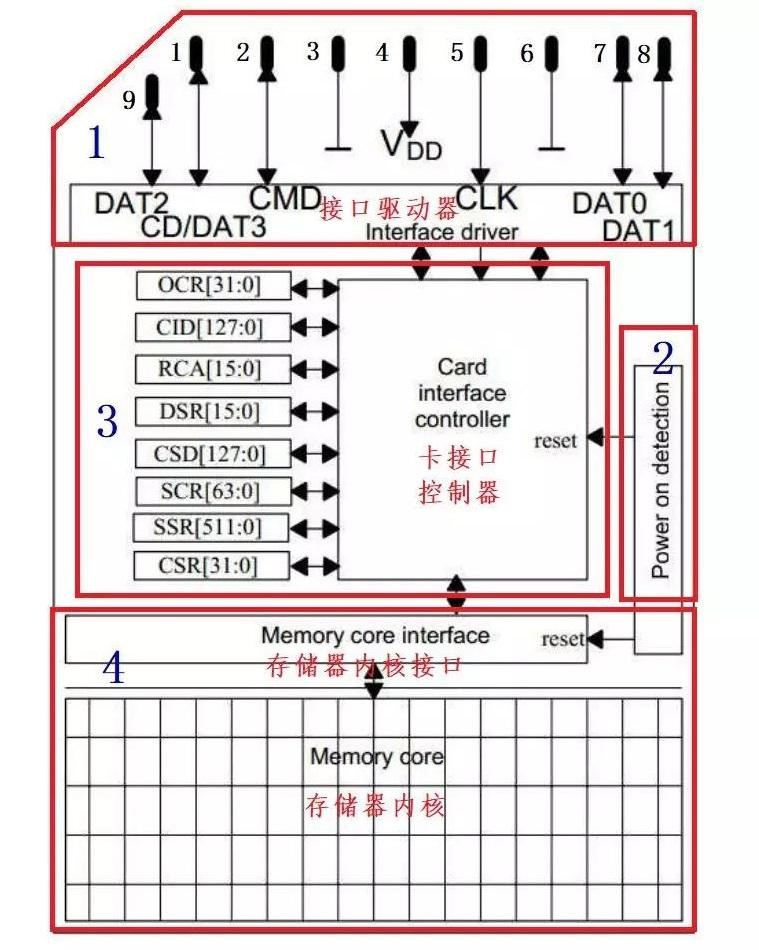
\includegraphics[width=0.5\textwidth]{figures/06-02-SD.jpg}
	\caption{SD卡内部结构}
\end{figure}

\subsubsection{什么是SDIO}

SDIO是在SD标准上定义了一种外设接口,它和SD卡规范间的一个重要区别是增加了低速标准。在SDIO卡只需要SPI和1位SD传输模式。低速卡的目标应用是以最小的硬件开销支持低速IO能力。

\subsubsection{什么是MCI}

MCI是Multimedia Card Interface的简称,即多媒体卡接口。上述的MMC,SD,SDI卡定义的接口都属于MCI接口。MCI这个术语在驱动程序中经常使用,很多文件,函数名字都包括“mci”。

\subsubsection{MMC/SD/SDIO卡的区别}

\begin{table}[h]
    \centering
\begin{tabular}{|c|c|c|c|}
    \hline
    卡属性&MMC卡&SD卡&SDIO卡\\
    \hline
    引脚个数&7&9&9\\
    \hline
    宽度&24mm&24mm&24mm\\
    \hline
    长度&32mm&32mm&32mm+\\
    \hline
    厚度&1.4mm&2.1mm&2.1mm\\
    \hline
    SPI传输模式&可选&支持&支持\\
    \hline
    一位传输模式&是&是&是\\
    \hline
    四位传输模式&否&可选&可选\\
    \hline
    时钟频率&0-20MHz&0-25MHz&0-25MHz\\
    \hline
    最高传输率&20Mbit/s&100Mbit/s&100Mbit/s\\
    \hline
    最高SPI传输率&20Mbit/s&25Mbit/s&25Mbit/s\\
    \hline
  \end{tabular}
  \caption{卡对比表}
\end{table}

SD卡内部有7个寄存器,如表6-2所示。其中OCR,CID,CSD和SCR寄存器保存卡的配置信息;RCA寄存器保存着通信过程中卡当前暂时分配的地址(只适合SD模式);卡状态(Card Status)和SD状态(SD Status)寄存器保存着卡的状态(例如,是否写成功,通信的CRC校验是否正确等),这两个寄存器的内容与通信模式(SD模式或SPI模式)相关。MMC卡没有SCR和SD Status寄存器。\\
\begin{table}[h]
    \centering
\begin{tabular}{|c|c|c|}    

    \hline
    名字	&宽度	&描述\\
    \hline
    CID	&128	&卡识别号,每张卡都有的唯一识别号\\
    \hline
    RCA	&16	&发布卡的地址,卡的局部系统地址,在初始化过程中,由主机和卡动态支持\\
    \hline
    DSR	&16&	驱动级寄存器,配置卡的驱动输出\\
    \hline
    CSD	&128&	卡的协议数据,关于卡的操作状态数据\\
    \hline
    SCR	&64	&卡配置寄存器,关于卡特性容量的信息\\
    \hline
    OCR	&32	&操作状态寄存器\\
    \hline
    SSR	&512&	SD状态,有关卡拥有的特性信息\\
    \hline
    CSR	&32	&卡状态,有关卡状态的信息\\
    \hline
\end{tabular}
\caption{卡寄存器表}
\end{table}

OCR寄存器保存着SD/MMC卡的供电电允许范围。如表6-3所示:如果OCR寄存器的某位为1,表示卡支持该位对应的电压。最后一位表示卡上电后的状态(是否处于“忙状态”),如果该位为0,表示忙,如果为1,表示处于空闲状态(MMC/SD协议P60)。\\

\begin{table}[h]
    \centering
\begin{tabular}{|c|c|}
    \hline
OCR~bit~position&VDD~votage~window\\
\hline
0-3	&Reserved\\
\hline
4	&1.6-1.7\\
\hline
5	&1.7-1.8\\
\hline
6	&1.8-1.9\\
\hline
7	&1.9-2.0\\
\hline
8	&2.0-2.1\\
\hline
9	&2.1-2.2\\
\hline
10	&2.2-2.3\\
\hline
11	&2.3-2.4\\
\hline
12	&2.4-2.5\\
\hline
13	&2.5-2.6\\
\hline
14	&2.6-2.7\\
\hline
15	&2.7-2.8\\
\hline
16	&2.8-2.9\\
\hline
17	&2.9-3.0\\
\hline
18	&3.0-3.1\\
\hline
19	&3.1-3.2\\
\hline
20	&3.2-3.3\\
\hline
21	&3.3-3.4\\
\hline
22	&3.4-3.5\\
\hline
23	&3.5-3.6\\
\hline
24-30	&Reserved\\
\hline
31	&Card~power~up~status~bit~(busy)1\\
\hline
\end{tabular}
\caption{电平-比特位表}
\end{table}

CID为一个16个字节的寄存器,该寄存器包含一个独特的卡标识号。

\begin{table}[!ht]
    \centering
\begin{tabular}{|c|c|c|c|}
    \hline
    Name	            &Field	&Width	&CID-slice\\
    \hline
    Manufacturer~ID	    &MID     &8	    &[127:120]\\
    \hline
    OEM/Application~ID	&OID     &18	    &[119:104]\\
    \hline
    Product~name	    &PNM	    &40	    &[103:64]\\
    \hline
    Product~Revision	&PRV     &8	    &[83:56]\\
    \hline
    Product~serial~number	&PSN &32	    &[55:24]\\
    \hline
    Reserved	        &...	    &4	    &[23:20]\\
    \hline
    Manufacturing~Date	&MDT     &12	    &[19:8]\\
    \hline
    CRC7~Checksum	    &CRC	    &7	    &[7:1]\\
    \hline
    not~used,~always~"T"&-	    &1	    &[0:0]\\
    \hline
\end{tabular}
\caption{卡识别号表}
\end{table}

SD/SDIO有以下几种传输模式:
\begin{itemize}
	\item SPI mode,独立序列输入和独立序列输出,使用CS、DI、SCLK与DO(SD卡的片选、数据输入、时钟与数据输出)四根信号线进行数据传输。
	\item 1-bit mode,独立指令和数据通道,只支持1位宽的数据传输。
	\item 4-bit mode,使用额外的针脚以及某些重新设置的针脚。支持四位宽的并行传输。
\end{itemize}

\subsection{K210联动SD卡}

K210 裸机使用SD卡,下图是SD卡对应接口:
\begin{figure}[H]
    \centering
    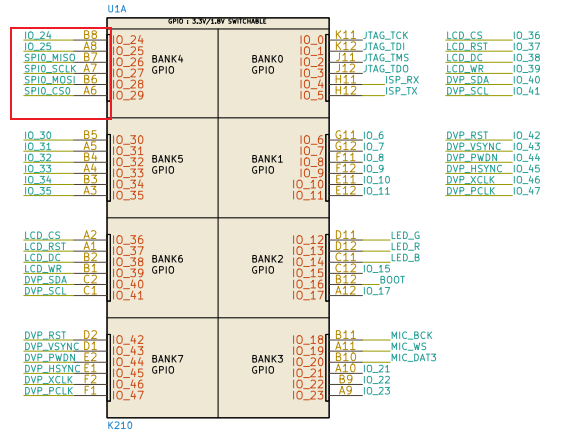
\includegraphics[width=0.8\textwidth]{figures/06-02-接口标.png}
    \caption{SD卡与K210接口}
\end{figure}

为了协同软硬接口,我们需要在代码中定义相关常量,使软硬接口保持一致,这即为遵守SD卡协议。
\begin{lstlisting}[language={Rust}, label={code:inode},
	caption={SD卡协议}]
    const MMIO =[
        (0x0C00_0000, 0x3000), /* PLIC */
        (0x0C20_0000, 0x1000), /* PLIC */
        (0x3800_0000, 0x1000), /* UARTHS */
        (0x3800_1000, 0x1000), /* GPIOHS */
        (0x5020_0000, 0x1000), /* GPIO */
        (0x5024_0000, 0x1000), /* SPI_SLAVE */
        (0x502B_0000, 0x1000), /* FPIOA */
        (0x502D_0000, 0x1000), /* TIMER0 */
        (0x502E_0000, 0x1000), /* TIMER1 */
        (0x502F_0000, 0x1000), /* TIMER2 */
        (0x5044_0000, 0x1000), /* SYSCTL */
        (0x5200_0000, 0x1000), /* SPI0 */
        (0x5300_0000, 0x1000), /* SPI1 */
        (0x5400_0000, 0x1000), /* SPI2 */
        ];
\end{lstlisting}


应用程序通过文件系统接口如open()、read()、write()、close()等访问文件系统,根据文件系统inode节点,接着找到文件在SD卡驱动上的块号。文件系统通过块设备驱动层与SD卡协议层对接,块设备驱动层定义了抽象块设备的接口,主要包括对块设备的读写接口。SD卡协议层主要负责按照SD卡标准规范向SD卡发送指令或者接收响应数据;硬件接口层则负责按照硬件板卡的引脚定义操作GPIO或SPI引脚实现与SD卡的数据交互。

\subsection{SD卡的命令}
SD卡命令共分为12类,分别为class0到Class11。


Class0:卡的识别、初始化等基本命令集
\begin{itemize}
	\item CMD0:复位SD 卡。
	\item CMD1:读OCR寄存器。
	\item CMD9:读CSD寄存器。
	\item CMD10:读CID寄存器。
	\item CMD12:停止读多块时的数据传输。
	\item CMD13:读 Card\_Status 寄存器。
\end{itemize}

Class2:读卡命令集
\begin{itemize}
	\item CMD16:设置块的长度。
	\item CMD17:读单块。
	\item CMD18:读多块,直至主机发送CMD12为止 。
\end{itemize}

Class4:写卡命令集
\begin{itemize}
	\item CMD24:写单块。
	\item CMD25:写多块。
	\item CMD27:写CSD寄存器 。
\end{itemize}

Class5:擦除卡命令集
\begin{itemize}
	\item CMD32:设置擦除块的起始地址。
	\item CMD33:设置擦除块的终止地址。
	\item CMD38: 擦除所选择的块。
\end{itemize}

Class6:写保护命令集
\begin{itemize}
	\item CMD28:设置写保护块的地址。
	\item CMD29:擦除写保护块的地址。
	\item CMD30: Ask the card for the status of the write protection bits。
\end{itemize}

Class7:卡的锁定,解锁功能命令集。

Class8:申请特定命令集 。

Class10 - 11:保留。

(注:完整细节请自行参考SD卡协议官方文档)。

\subsection{SD卡工作流程}

SD卡工作流程大致可以分为3个大的步骤:初始化SD卡、写SD卡、读SD卡。在SPI模式下,SD卡工作模式分为卡识别模式和数据传输模式。如下图为卡在识别模式下的命令流程。

\begin{figure}[H]
    \centering
    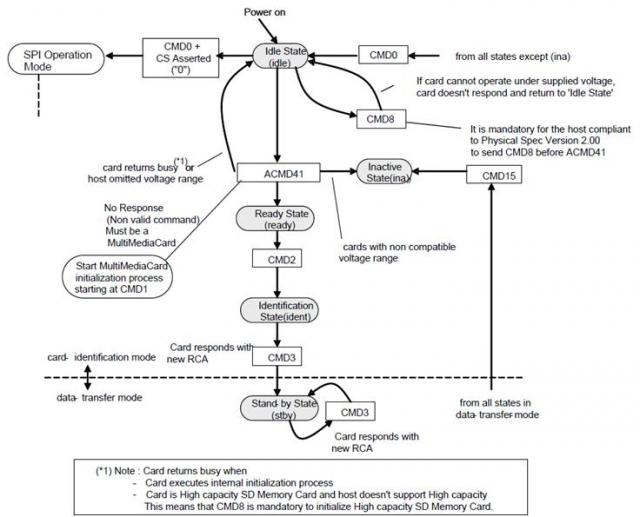
\includegraphics[width=0.8\textwidth]{figures/06-02-命令流程.png}
    \caption{SD卡识别模式命令流程}
\end{figure}


在复位后,查找总线上的新卡的时候,主机会处于“卡识别模式”。卡在复位后会处于识别模式。不同的SD卡可能支持不同版本的协议或者不同的⼯作电压。因此,作为主机,在与SD卡进行交互之初,主机需要获取卡的工作电压范围和卡的类型。在卡识别期间,时钟频率应该保持在100 - 400kHZ之间。

\begin{enumerate}
	\item 在主机和SD卡进行任何通信之前,主机不知道SD卡支持的工作电压范围,卡也不知道是否支持主机当前提供的电压。因此主机首先使用默认的电压发送一条reset指令(CMD0)。
	\item 为了验证SD卡的接口操作状态,主机发送SEND\_IF\_COND(CMD8),用于取得SD卡支持工作的电压范围数据。SD卡通过检测CMD8的参数部分来检查主机使用的工作电压,主机通过分析回传的CMD8参数部分来校验SD卡是否可以在所给电压下工作,如果SD卡可以在指定电压下工作,则它回送CMD8的命令响应字 。如果不支持所给电压,则SD卡不会给出任何响应信息,并继续处于IDLE状态。
	\item 在发送ACMD41命令初始化高容量的SD卡前,需要强制发送CMD8命令。强制低电压主机在发送CMD8前发送ACMD41,万一双重电压SD卡没有收到CMD8命令且工作在高电压状态,在这种情况下,低电压主机不能不发送CMD8命令给卡,则收到ACMD41后进入无活动状态。
	\item SD\_SEND\_OP\_COND(ACMD)命令是为SD卡主机识别卡或者电压不匹配时拒绝卡的机制设计的。主机发送命令操作数代表要求的电压窗口大小。如果SD卡在所给的范围内不能实现数据传输,将放弃下一步的总线操作而进入无活动。操作状态寄存器也将被定义。
	\item 在主机发出复位命令(CMD0)后,主机将先发送CMD8再发送ACMD41命令重新初始化SD卡。
\end{enumerate}

当总线被激合后,主机就开始卡的初始化和识别3处理。初始化处理设置它的操作状态和是设置OCR中的HCS比特命令SD\_SEND\_OP\_COND(ACMD41)开始。HCS比特位被设置为1表示主机支持高容量SD卡。HCS被设置为0表示主机不支持高容量SD卡。卡的初始化和识别流程见下图。

\begin{figure}[H]
    \centering
    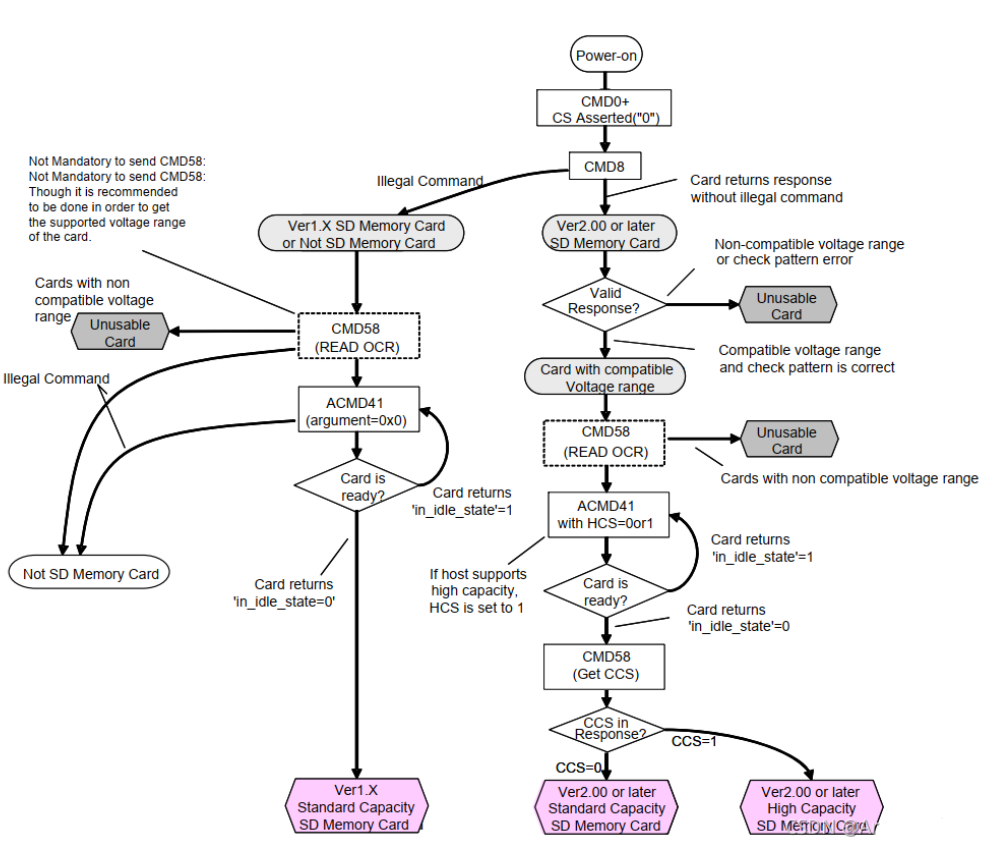
\includegraphics[width=0.8\textwidth]{figures/06-02-初始化.png}
    \caption{卡初始化和识别流程}
\end{figure}
(注:这里不推荐使用NPUCore或rCore作为代码范式来讲解,应直接看SD卡协议文档)

卡在识别模式结束后,主机时钟fpp(数据传输时钟频率)将保存为fod(卡识别模式下的时钟),由于有些卡对操作时钟有限制。主机必须发送SEND\_CSD(CMD9)来获得卡规格数据积存器内容,如块大小,卡容量。广播命令SET\_DSR(CMD4)配置所有识别卡的驱动阶段。它对DSR积存器进行编程以适应应用总线布局,总线上的卡数目和数据传输频率。SD卡数据传输模式的流程图如下图。
\begin{figure}[H]
    \centering
    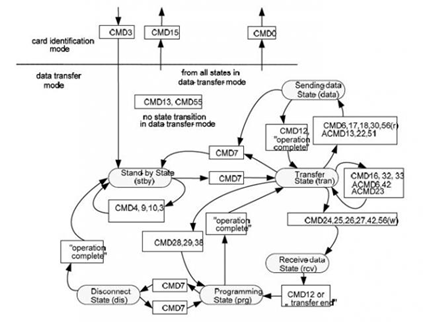
\includegraphics[width=0.8\textwidth]{figures/06-02-数据传输.png}
    \caption{SD卡数据传输模式流程}
\end{figure}

\begin{enumerate}
	\item CMD7命令用来选择某个SD卡,使其进入Transfer状态,在指定时间段内,只有一个卡能处于Transfer状态。当某个先前被选中的处于Transfer状态的SD卡接收到CMD7之后,会释放与控制器的连接,并进入Stand-by态。当CMD7使用保留地址0x0000时,所有的SD卡都会进入Stand-by状态。
	\item 所有的数据读命令都可以被停止命令(CMD12)在任意时刻终止。数据传输会终止,SD卡返回Transfer状态。读命令有:块读操作(CMD17)、多块读操作(CMD18)、发送写保护(CMD30)、发送scr(ACMD51)以及读模式下的普通命令(CMD56)。
	\item 所有的数据写命令都可以被停止命令(CMD12)在任意时刻终止。写命令也会在取消选择命令(CMD7)之前停止。写命令有:块写操作(CMD24,CMD25)、编程命令(CMD27)、锁定/解锁命令(CMD42)以及写模式下的普通命令(CMD56)。
	\item 数据传输一旦完成,SD卡会退出数据写状态,进入Programming状态(传输成功)或者Transfer状态(传输失败)。
\end{enumerate}
\clearpage